\documentclass{fkbook}

% For resolution of that one triangulation
\usetikzlibrary{intersections}

% For the tetrahedron thing
\usetikzlibrary{backgrounds}

% For 3d plots
\usepackage{tikz-3dplot}

\usetikzlibrary{external}
\tikzexternalize
\tikzsetexternalprefix{figures/}

\usepackage{fkthm}
% For music note in subtitle

\usepackage{wasysym}

\begin{document}

\pagestyle{plain}
\frontmatter

\fkauthor{Forest Kobayashi}
\fktitle{Homology Theory}
\fksubtitle{Notes \& Exercises from my Independent Study}
\fkalttitle{(Or: \itshape If I could save Klein in a bottle \eighthnote)}
\fkaffiliation{{Department of Mathematics\\}{\itshape Harvey Mudd College\\}}
\fksupervisor{Francis Su}
\fksupervisoraffiliation{Department of Mathematics, Harvey Mudd College}

\maketitlepage
\tableofcontents

\chapter{Introduction}
\section*{What's this?}\noindent\indent
This document is a compendium of notes, exercises, and other miscellany from my
independent study in Homology Theory. For this, I am working through the second
half of \emph{Topology Through Inquiry} by Michael Starbird and Francis Su
(i.e., chapters 11-20), under supervision from Prof.\ Su himself. Rough topic
coverage should be discernable from the table of contents, as I've tried to
name each section identically to the corresponding title in the book.

\section*{Notation}
Most notation I use is fairly standard. Here's a (by no means exhaustive) list
of some stuff I do.
\begin{itemize}
  \item ``WTS'' stands for ``want to show,'' $\st$ for ``such that.'' WLOG, as
    usual, is without loss of generality.
  \item End-of-proof things: $\blacksquare$ is QED for exercises and theorems.
    $\square$ is used in recursive proofs (e.g., proving a Lemma within a
    theorem proof). If doing a proof with casework, $\cmark$ will be used to
    denote the end of each case.
  \item \contra\ means contradiction
  \item $\mathscr{T}(U)$ will denote the topology of a topological space $U$.
  \item $\mc P(A)$ is the powerset of $A$. I don't like using $2^A$.
  \item $\onto$ denotes surjection.
  \item $\into$ denotes injection.
  \item Thus, $\bij$ denotes bijection.
  \item \textbf{Important:} I use $f\fim[A]$ for the image of $A$ under $f$, and
    $f\fpre[B]$ for the inverse image of $B$ under $f$.
  \item $\sim$ and $\equiv$ are used for equivalence relations. $\cong$ is used
    to denote homeomorphism and isomorphism of groups. $\simeq$ is for Homotopy
    equivalence.
  \item $\epsilon$ is for trivial elements (e.g., the trivial path), while
    $\varepsilon$ is for small positive quantities.
  \item $\ol{U}$ denotes the closure of $U$, $\interior{U}$ is the interior of
    $U$.
  \item $A^c$ is $A$ complement.
  \item $\simp{k}$ denotes a simplex on $k+1$ vertices (that is, a $k$-simplex).
    $\simpdel{i}{k}$ is the same simplex with the $i$\textsuperscript{th} vertex
    deleted.
  \item $[n] = \set{i \MID i = 0,1,\ldots, n}$.
\end{itemize}

\mainmatter

\pagestyle{main}

\chapter[Homological Prereqs]{Manifolds, Simplexes Complexes, and Triangulability: Building Blocks}

\section{Manifolds}
We define some basic Euclidean sets for use in homeomorphisms.
\begin{definition}
  The \emph{$n$-dimensional cube}, denoted $\DD^n$, is defined as
  \begin{align*}
    \DD^n
    &= \set{\pn{x_1, \ldots, x_n} \in \RR^n \MID 0 \leq x_i \leq 1 \text{ for } i = 1, \ldots, n} \\
    &= \overbrace{[0,1] \times [0,1] \times \cdots \times [0,1]}_{n \text{ times}} \subset \RR^n.
  \end{align*}
\end{definition}
\begin{definition}
  The \emph{standard $n$-ball}, denoted $B^n$, is
  \[
    B^n = \set{\pn{x_1, \ldots, x_n} \in \RR^n \MID x_1^2 + \cdots + x^2_n \leq
      1}.
  \]
\end{definition}
\begin{definition}
  The \emph{standard $n$-sphere}, denoted $\Ss^n$, is
  \[
    \Ss^n = \set{(x_0, \ldots, x_n) \in \RR^{n+1} \MID x^2_0 + \cdots + x^2_n =
      1}.
  \]
  note that here, our indices start at $0$.
\end{definition}
\begin{definition}
  An \emph{$n$-dimensional manifold} or \emph{$n$-manifold} is a separable
  metric space $M$ such that $\forall p \in M$, $\exists U \in \ms T(M) \st p
  \in U$ and $U \cong V \subset \RR^n$.
\end{definition}
\begin{problem}[15.8]
  If $M$ is an $n$-manifold and $U$ is an open subset of $M$, then $U$ is also
  an $n$-manifold.
\end{problem}
\begin{proof}

\end{proof}
\begin{problem}[15.9]
  If $M$ is an $m$-manifold and $N$ is an $n$-manifold, then $M \times N$ is an
  $(m+n)$-manifold.
\end{problem}
\begin{proof}

\end{proof}
\begin{problem}[15.10]
  Let $M^n$ be an $n$-dimensional manifold with boundary. Then $\partial M^n$ is
  an $(n-1)$-manifold.
\end{problem}
\begin{proof}

\end{proof}
\section{Simplicial Complexes}~
\begin{definition}[Affine Independence]
  Let $X = \set{v_0, \ldots, v_k} \subset \RR^n$. We say $X$ is \emph{affinely
    independent} if $\set{v_1 - v_0, \ldots, v_k - v_0}$ is linearly
  independent.
\end{definition}

%%% Local Variables:
%%% TeX-master: "main"
%%% End:
\chapter{Simplicial $\ZZ_2$-Homology: Physical Algebra}
\section{Intro}
This chapter, we'll talk about \emph{homology}, which captures holes in a much
more satisfying way than higher homotopy groups do.
\begin{adjustwidth}{1.5em}{}
  \begin{remark}
    Although not exactly accurate, a good way to start to understand homology for
    a space $X$ is to view an $n$-manifold in $X$ that is not the boundary of an
    $(n+1)$-manifold-with-boundary as capturing some geometry of $X$ while an
    $n$-manifold that is the boundary of an $(n+1)$-dimensional
    manifold-with-boundary is not detecting any hole or structure.
  \end{remark}
\end{adjustwidth}
\section{Chains, Cycles, Boundaries, and the Homology Groups}
\begin{definition}
  An \emph{$n$-chain} of $K$ is a finite formal sum
  \[
    \sum_{i=1}^k \sigma_i
  \]
  of distinct $n$-simplices in $K$. Note that the dimensions of the simplices
  must be the same. So \emph{chain} will mean $n$-chain whenever the dimension
  is either unimportant or understood.
\end{definition}
\begin{definition}
  The \emph{$n$-chain group of $K$} (with coefficients in $\zmod{2}$), denoted
  $\mathsf{C}_n(K)$, is the collection of $n$-chains in $K$ under formal
  addition modulo 2. If there are no $n$-simplices in $K$, the $n$-chain group
  of $K$ is defined to be trivial (containing the ``empty'' chain).
\end{definition}
\begin{problem}[16.1]
  Check that $\msf C_n(K)$ is an abelian group.
\end{problem}
\begin{solution}
  \begin{enumerate}[label=(\arabic*)]
    \item $\epsilon = \sum_{i \in \varnothing} \sigma_i$.
    \item Associativity inherited from $\cup$.
    \item Closure inherited from $\cup$ over the domain given.
    \item Existence of inverses --- since we're taking formal linear
      combinations over $\zmod{2}$, then every element is its own inverse.
  \end{enumerate}
  Finally, to see that $\msf C_n(K)$ is abelian, observe that $+$ in $\msf
  C_n(K)$ inherits commutativity from $\cup$.
\end{solution}
\begin{definition}
  The \emph{$\zmod{2}$-boundary of an $n$-simplex $\sigma = \simp{n}$} is
  defined by
  \[
    \partial \sigma = \sum_{i=0}^n \simpdel{i}{n}
  \]
  the formal sum of the $(n-1)$-faces of $\sigma$.

  For a 0-simplex, the $\zmod{2}$ boundary is defined to be $0 \in \msf
  C_{-1}(K)$.
\end{definition}
\begin{definition}
  The \emph{$\zmod{2}$ boundary of an $n$-chain} is the sum of the boundaries of
  the simplices. That is, $\partial_n : \msf C_n(K) \to \msf C_{n-1}(K)$ is
  given by
  \[
    \partial\pn{\sum_{i=1}^k \sigma_i} = \sum_{i=1}^k \partial(\sigma_i)
  \]
\end{definition}
\begin{problem}[16.2]
  Verify that $\partial$ is a homomorphism, and use the definition to compute
  the $\zmod{2}$ boundary of $\sigma_1 + \sigma_2$ in Figure 16.1
\end{problem}
\begin{solution}
  The homomorphism is straightforward. $\partial(\sigma_1 + \sigma_2) = e_1 +
  e_2 + e_4 + e_5$.
\end{solution}
\begin{definition}
  An \emph{$n$-cycle} is an $n$-chain of $K$ whose boundary is zero. The set of
  all $n$-cycles on $K$ is denoted $\msf Z_n(K)$. An \emph{$n$-boundary} is an
  $n$-chain that is the boundary of an $(n+1)$-chain of $K$. The set of all
  $n$-boundaries is denoted $\msf B_n(K)$.
\end{definition}
% \begin{problem}[16.3]

% \end{problem}
\begin{problem}[16.4]
  Both $\msf Z_n(K)$ and $\msf B_n(K)$ are subgroups of $\msf C_n(K)$. Moreover,
  \[
    \partial \circ \partial = 0.
  \]
  In other words, $\partial_n \circ \partial_{n+1} = 0$ foreach index $n \geq
  0$. Hence, $\msf B_n(K) \subset \msf Z_n(K)$.
\end{problem}
\begin{solution}
  Let $\sigma_1, \sigma_2 \in \msf Z_n(K)$. Then by linearity of $\partial_n$,
  we have
  \begin{align*}
    \partial_n(\sigma_1 + \sigma_2)
    &= \partial_n(\sigma_1) + \partial_n(\sigma_2) \\
    &= 0
  \end{align*}
  and hence $\msf Z_n(K) < \msf C_n(K)$.

  Now, let $\sigma_1, \sigma_2 \in \msf B_n(K)$. Then $\exists \tau_1, \tau_2
  \in \msf Z_{n+1}(K)$ such that $\partial_{n+1}(\tau_1) = \sigma_1,
  \partial_{n+1}(\tau_2) = \sigma_{2}$. Then by linearity of $\partial$, we have
  \begin{align*}
    \partial_{n+1}(\tau_1 + \tau_2)
    &= \partial_{n+1}(\tau_1) + \partial_{n+1}(\tau_2) \\
    &= \sigma_1 + \sigma_2
  \end{align*}
  hence $\msf B_n(K)$ is a subset closed under the operation, so we have $\msf
  B_n(K) < \msf C_n(K)$.
\end{solution}
\begin{definition}
  Two $n$-cycles $\alpha$ and $\beta$ in $K$ are \emph{equivalent} or
  \emph{homologous} iff $\alpha-\beta = \partial(\gamma)$ for some $(n+1)$-chain
  $\gamma$. In other words, $\alpha$ and $\beta$ are homologous iff they differ
  by an element of the subgroup $\msf B_n(K)$, denoted by
  \[
    \alpha \sim_{\zmod{2}} \beta.
  \]
  The equivalence class of $\alpha$ is denoted by enclosing it in brackets
  thusly: $[\alpha]$. For $\zmod{2}$ $n$-chains, observe that $\alpha - \beta =
  \alpha + \beta$. So we see that two $n$-cycles are equivalent if together they
  bound an $(n+1)$-chain.
\end{definition}
\begin{problem}[16.5]
  List all the equivalence classes of $0$-cycles, 1-cycles, and 2-cycles in the
  complex in Figure 16.1.
\end{problem}
\begin{solution}

\end{solution}
%%% Local Variables:
%%% TeX-master: "main"
%%% End:
\chapter{Some Homological Algebra}
The big idea: algebraic topology assigns discrete algebraic invariants to
topological spaces and continuous maps. Book for this section: James May's
\emph{A Concise Course in Algebraic Topology}

\section{Chain complexes}
\begin{definition}[Chain/Cochain Complexes]
  Let $R$ be a commutative ring. A \emph{chain complex} over $R$ is a sequence
  of maps of $R$-modules
  \[
    \cdots \rightarrow X_{i+1} \xrightarrow{d_{i+1}} X_i \xrightarrow{d_i}
    X_{i-1} \rightarrow \cdots
  \]
  such that $d_i \circ d_{i+1} = 0$ for all $i$. We generally abbreviate $d =
  d_i$. A \emph{cochain complex} over $R$ is an analogous sequence
  \[
    \cdots \rightarrow Y^{i-1} \xrightarrow{d^{i-1}} Y^i \xrightarrow{d^i}
    Y^{i-1} \rightarrow \cdots
  \]
  with $d^i \circ d^{i-1}$.

  We usually require chain complexes to satisfy $X_i = 0$ for $i < 0$, and
  cochain complexes to satisfy $Y^i = 0$ for $i < 0$. Without this distinction,
  the definitions are equivalent.
\end{definition}
\begin{definition}[Some definitions]
  Elements of $\ker d_i$ are called cycles. Elements of $\im d_{i+1}$ are called
  boundaries. Write $B_i(X) \subset Z_i(X) \subset X_i$ for the submodules of
  boundaries and dycles, and define the $i$\textsuperscript{th} homology group
  $H_i(X)$ by
  \[
    H_i(X) = Z_i(X) / B_i(X).
  \]
  We write $H_*(X)$ for the sequence of $R$-modules $H_i(X)$. We understand
\end{definition}

%%% Local Variables:
%%% TeX-master: "../main"
%%% End:
\chapter{Rotman}
The big idea: algebraic topology assigns discrete algebraic invariants to
topological spaces and continuous maps. Book for this section: Joseph Rotman's
\emph{A First Course in Algebraic Topology}

\section{A sketch of the Brouwer Fixed Point Theorem}
\begin{problem}[R 0.1]
  Every continuous function $f : D^1 \to D^1$ has a fixed point.
\end{problem}
\begin{solution}
  We'll prove this without the techniques of analysis, so as to make the
  connection to the general argument slightly more obvious. Let $f(-1) = a$ and
  $f(1) = b$.
  \begin{enumerate}[label=(\arabic*)]
    \item Suppose $a = -1$ or $b = 1$, then we're done.
    \item Else, $a > -1$ and $b < 1$. Consider the graph of $f$:
      \[
        G = \set{\pn{x, f(x)} \MID x \in D^1}
      \]
      since $f$ is continuous and $D^1$ is connected, $G$ is connected as well.
      Let
      \[
        A = \set{\pn{x, f(x)} \MID f(x) > x} \qquad \text{and} \qquad B =
        \set{\pn{x, f(x)} \MID f(x) < x}.
      \]
      \begin{figure}[H]
        \centering
        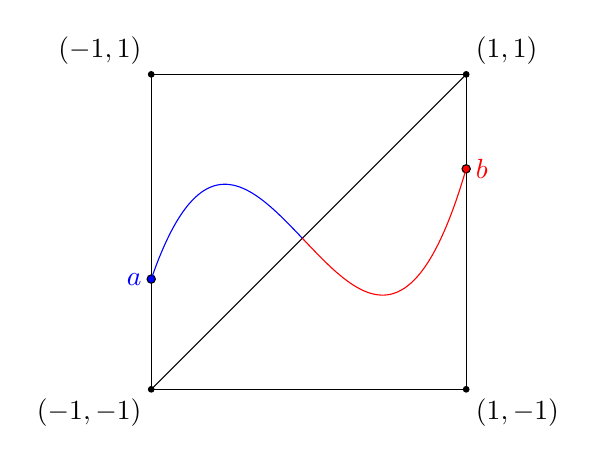
\begin{tikzpicture}[scale=2]
          \path
          coordinate (1) at (-1,-1)
          coordinate (2) at (-1,1)
          coordinate (3) at (1,1)
          coordinate (4) at (1,-1)
          coordinate (a) at (-1,-.3)
          coordinate (b) at (1, .4);

          \foreach \v in {1,2,3,4}{
            \draw[fill=black] (\v) circle (0.5pt);
          }

          \node[below left] (11) at (1) {$(-1,-1)$};
          \node[above left] (21) at (2) {$(-1,1)$};
          \node[above right] (31) at (3) {$(1,1)$};
          \node[below right] (41) at (4) {$(1,-1)$};

          \draw (1) -- (2) -- (3) -- (4) -- (1);
          \draw (1) -- (3);

          \draw[fill=blue] (a) circle (0.75pt);
          \draw[fill=red] (b) circle (0.75pt);
          \node[left] (ap) at (a) {$\color{blue}a$};
          \node[right] (bp) at (b) {$\color{red}b$};

          % \draw[domain=-1:1,smooth,variable=\x,blue] plot ({\x},{(-24 - 101*\x + 27*\x^2 + 122*\x^3)/60});
          \draw[domain=-1:-0.0405889,smooth,variable=\x,blue] plot ({\x},{\x*(\x*(1.4*\x + 0.133333) - 1.05) - 0.0833333});
          \draw[domain=-0.0405889:1,smooth,variable=\x,red] plot ({\x},{\x*(\x*(1.4*\x + 0.133333) - 1.05) - 0.0833333});

        \end{tikzpicture}
        \caption{$G$}
        \label{fig:brouwer-1}
      \end{figure}
      And let $\Delta = \set{\pn{x,x} \MID x \in [0,1]}$. Note $a \in A$, and $b
      \in B$, so $A \neq \varnothing \neq B$.

      Suppose $G \cap \Delta = \varnothing$. Then $G = A \sqcup B$. Note $A,B$
      are open in $G$, hence $G$ is not connected, a contradiction.
  \end{enumerate}
\end{solution}

\begin{definition}[retract]
  A subspace $X$ of a topological space $Y$ is a \emph{retract} of $Y$ if there
  is a continuous map $r : Y \to Y$ with $r(x) = x$ for all $x \in X$. Such a
  map is called a \emph{retraction}.
\end{definition}

% \begin{problem}[R 0.2]
%   If $n \geq 0$, then $S^n$ is not a retract of $D^{n+1}$
% \end{problem}
% \begin{solution}

% \end{solution}

\begin{problem}

\end{problem}

%%% Local Variables:
%%% TeX-master: "../main"
%%% End:

\chapter{Appendix}
\section{List of Definitions}
\listofdefinitions

\end{document}
%%% Local Variables:
%%% TeX-master: t
%%% TeX-engine: default-shell-escape
%%% TeX-command-extra-option: -pdf
%%% End: